\documentclass[11pt,a4paper]{extarticle}
\usepackage[margin=2cm, top=2cm, bottom=2cm]{geometry}
\usepackage{xeCJK}
\setCJKmainfont{Noto Serif CJK TC}[Script=CJK]
\usepackage{amsmath}  % 添加 amsmath 用於矩陣
\usepackage{fancyhdr}
\usepackage{graphicx}
\usepackage{hyperref}
\usepackage{url} % 支援 \url{}
\usepackage{booktabs} % 確保使用 booktabs 宏包
\usepackage{tabularx} % 讓表格寬度自適應
\usepackage{svg}
\usepackage{float}
\usepackage{indentfirst}  % 讓第一段也縮排
\setlength{\parindent}{2em} % 設定縮排 2 字寬


\setCJKmainfont{Noto Sans Mono CJK TC}

\linespread{1.2}\selectfont

\pagestyle{fancy}
\fancyhf{} % 清空頁眉頁腳設置****
\cfoot{\thepage} % 頁碼位於底部中間

\begin{document}

\section*{HW1.Decision Tree}
\lhead{HW1.Decision Tree}
\rhead{B12508026戴偉 璿}

    \section*{Tree Structure}
    \begin{figure}[H]
        \centering
        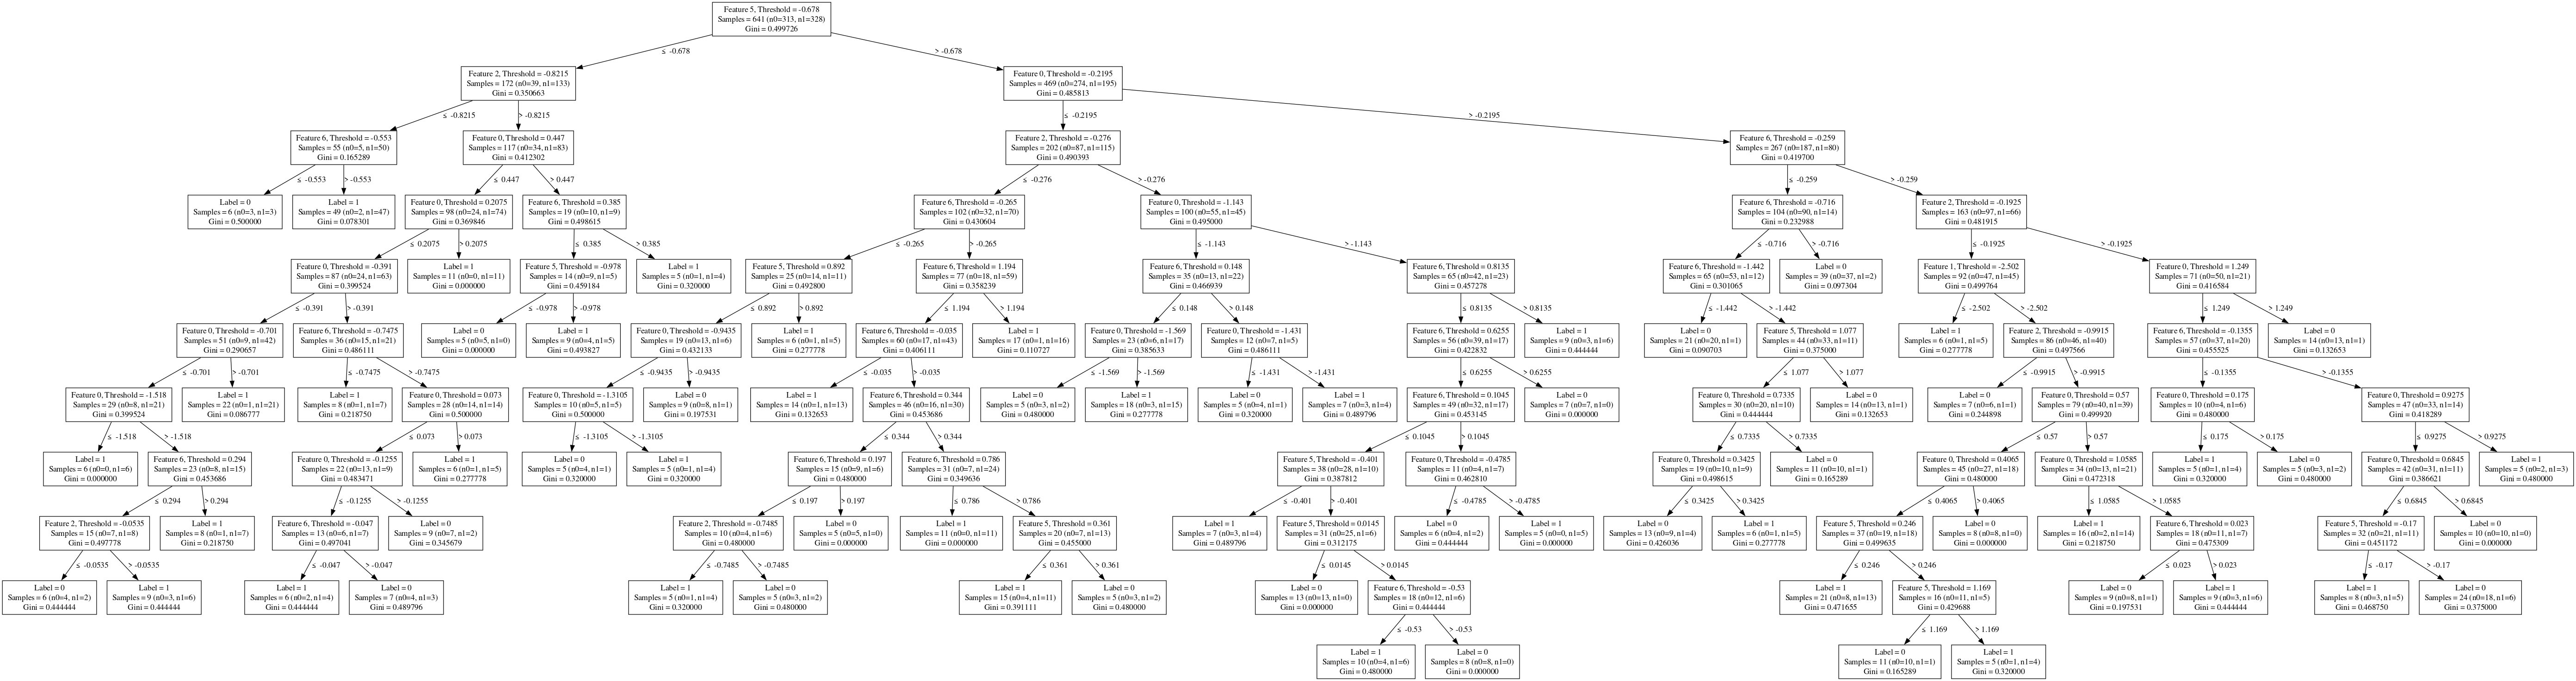
\includegraphics[width=0.8\textwidth]{src/tree_structure.png}
        \caption{Tree Structure}
    \end{figure}

    \section*{Discussion}
    \begin{enumerate}
        \item 圖片若模糊不清可參考資料夾中的「tree\_structure.svg」
        \item 決策樹參數:max\_depth=10, min\_leaves=5,準確率為83.6193\%
        \item Figure 2是不同最小子葉、最大深度測試結果的折線圖,詳細表格可以參考附錄中的 Table~\ref{tab1}。

            \begin{figure}[H]
                \centering
                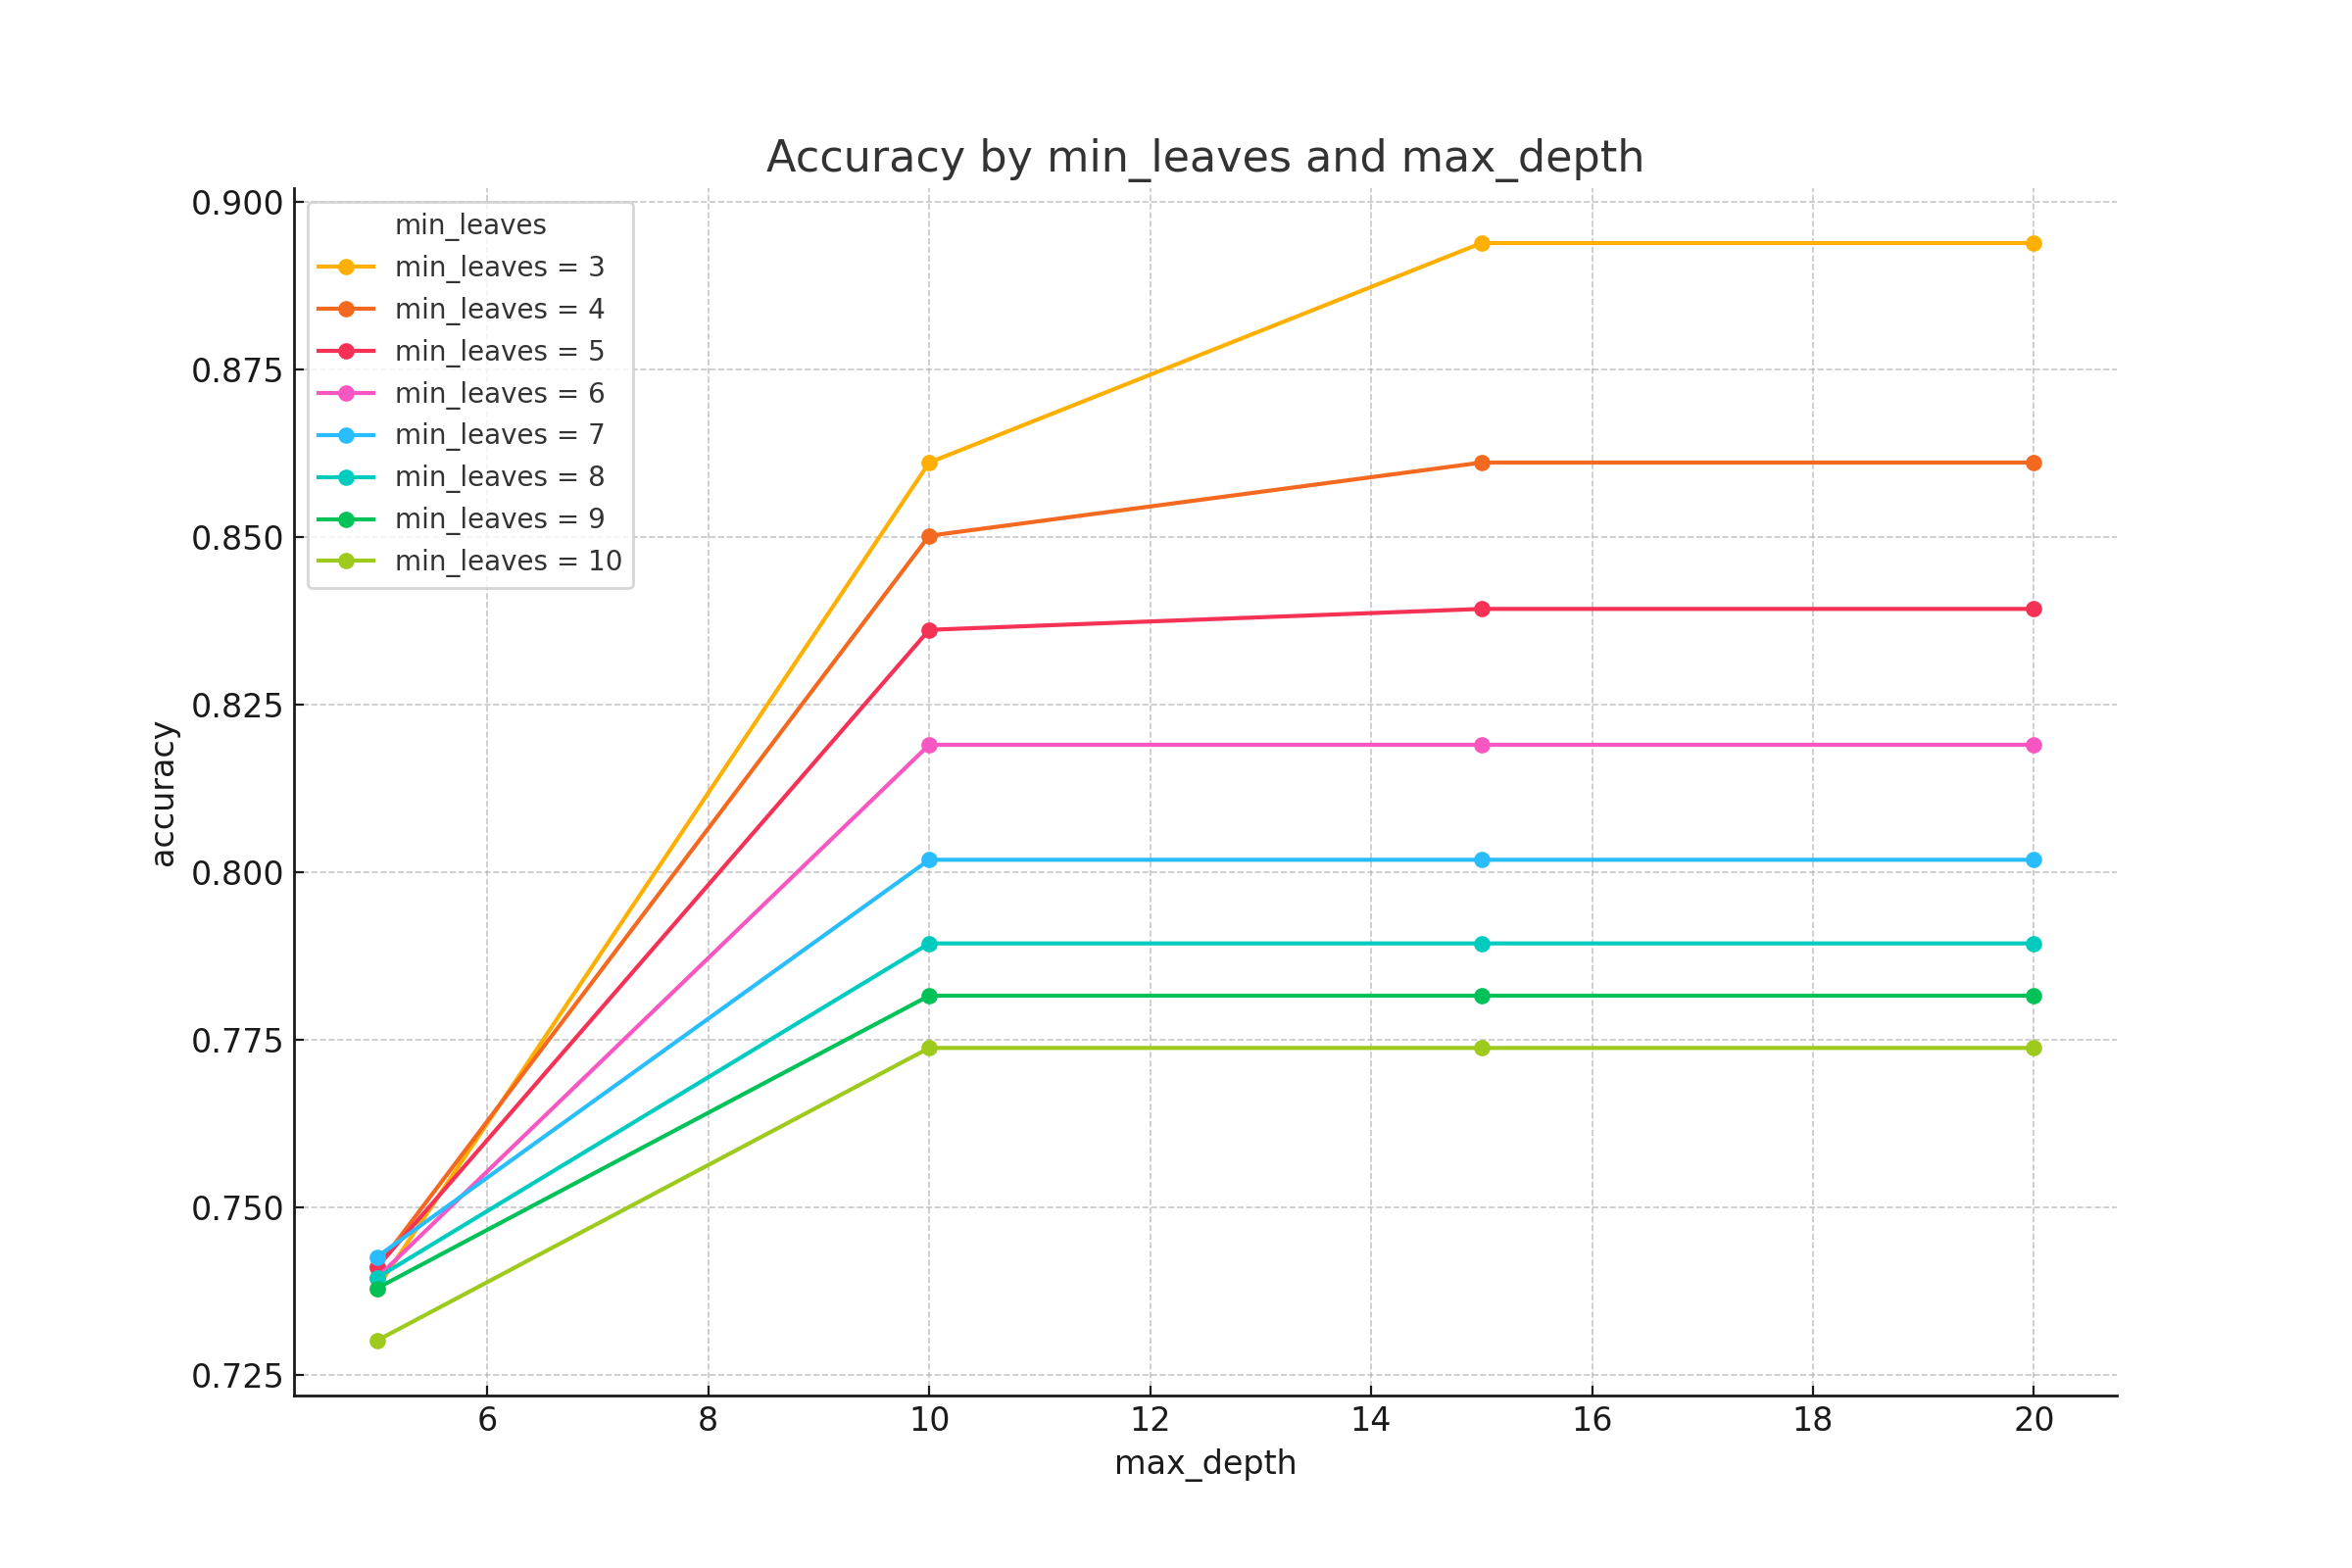
\includegraphics[width=0.8\textwidth]{src/picture1.png}
                \caption{訓練資料與測試資料相同}
            \end{figure}
        \newpage      
    \end{enumerate}

    可以發現,在最小子葉數為3,最大深度為20時,準確率有最高的89.39\%,準確率極高,但這樣的模型可能會過擬合。

    於是我又進行了一個測試:隨機取用620筆資料訓練,20筆資料測試且完全不重複(測試資料儲存在testdatas資料夾,使用gen.cpp生成),
    在每組不同最小子葉數、最大深度的組合都進行20次測試,取其平均值以求精確。結果如Table~\ref{tab2},
    結果折線圖如Figutre3:
    \begin{figure}[H]
        \centering
        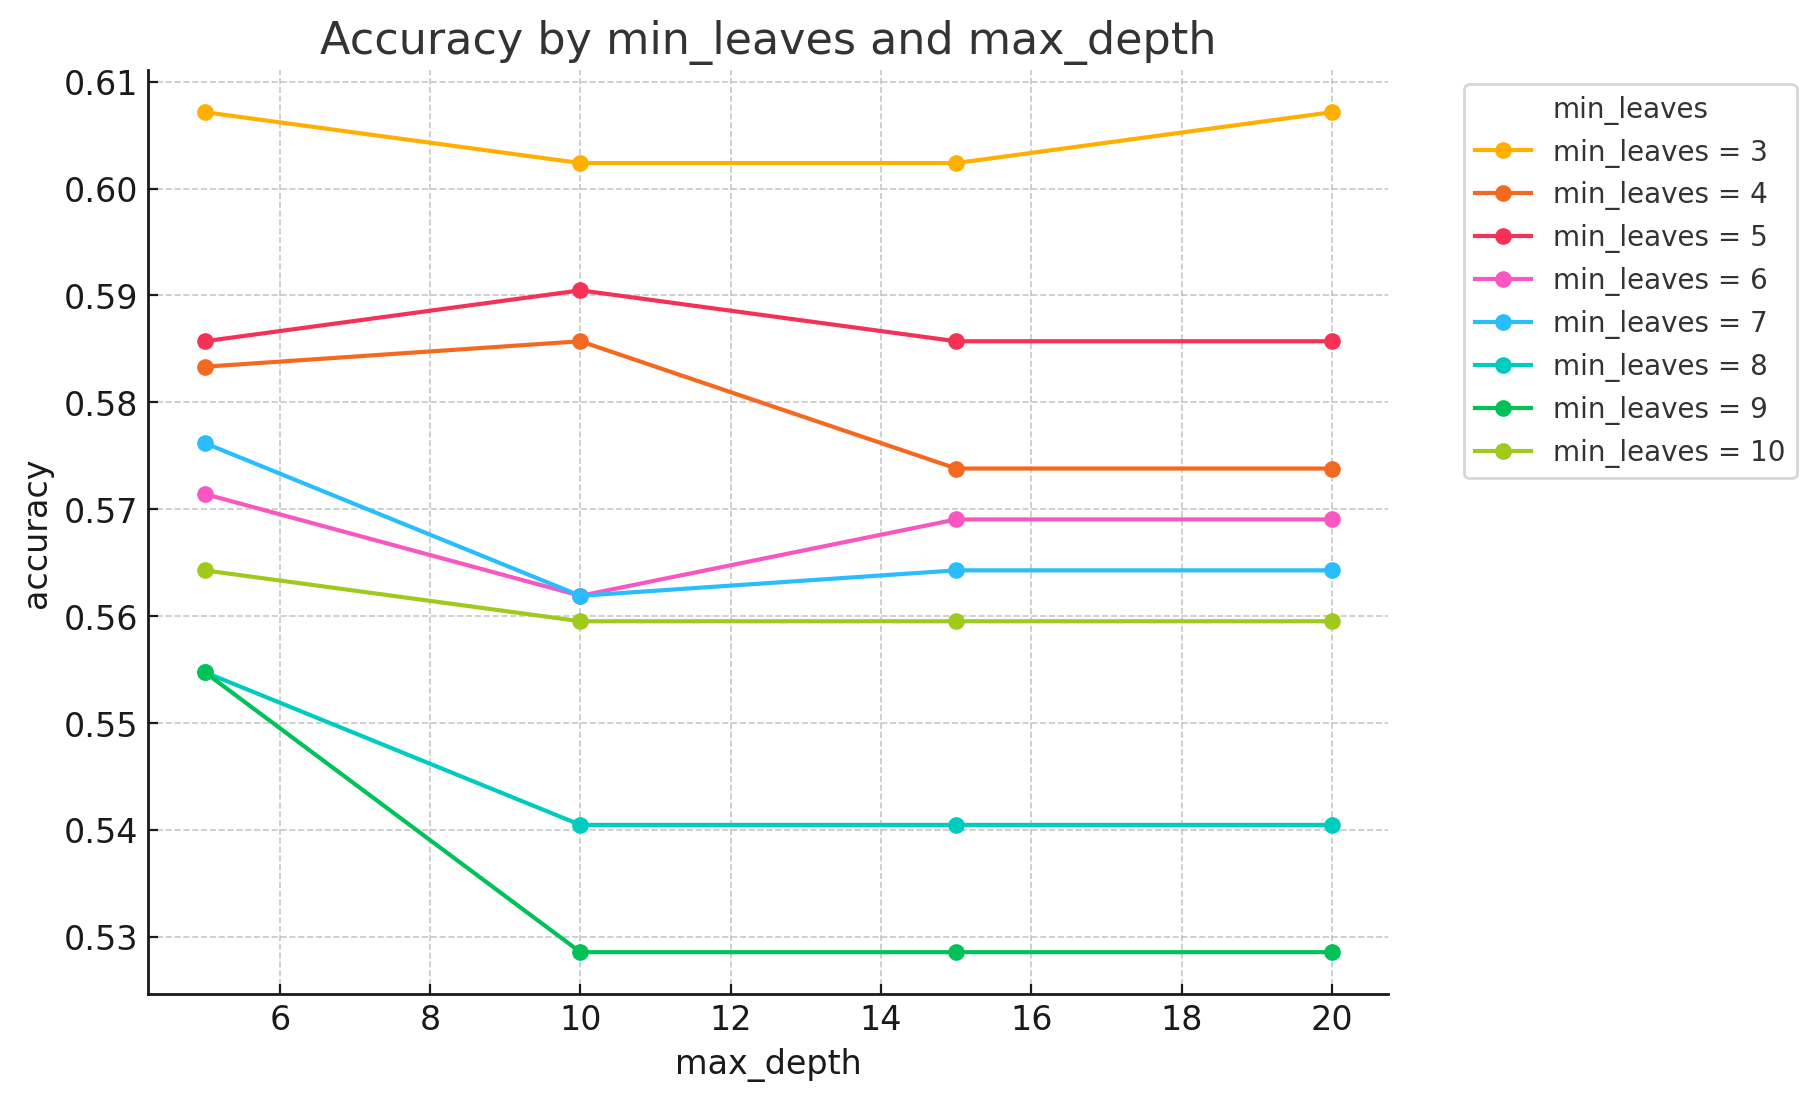
\includegraphics[width=0.8\textwidth]{src/picture2.png}
        \caption{訓練資料與測試資料完全不同}
    \end{figure}

    最高的準確率為60.71\%,和原本的結果差距極大,顯然是過擬合的問題。

    \newpage
    \section*{How to improve accuracy} 
    解決過擬合的方法有很多,例如增加訓練資料、減少特徵數、增加正則化等。但在測試資料有限的狀況下,我選擇使用隨機森林來解決過擬合的問題:
    建構多棵決策樹,並將每棵決策樹的結果進行投票,最後選擇投票最多的結果作為最終結果。

    以下是隨機森林測試的結果,表格資料可以參考附錄中的 Table~\ref{tab3}:

    \begin{figure}[H]
        \centering
        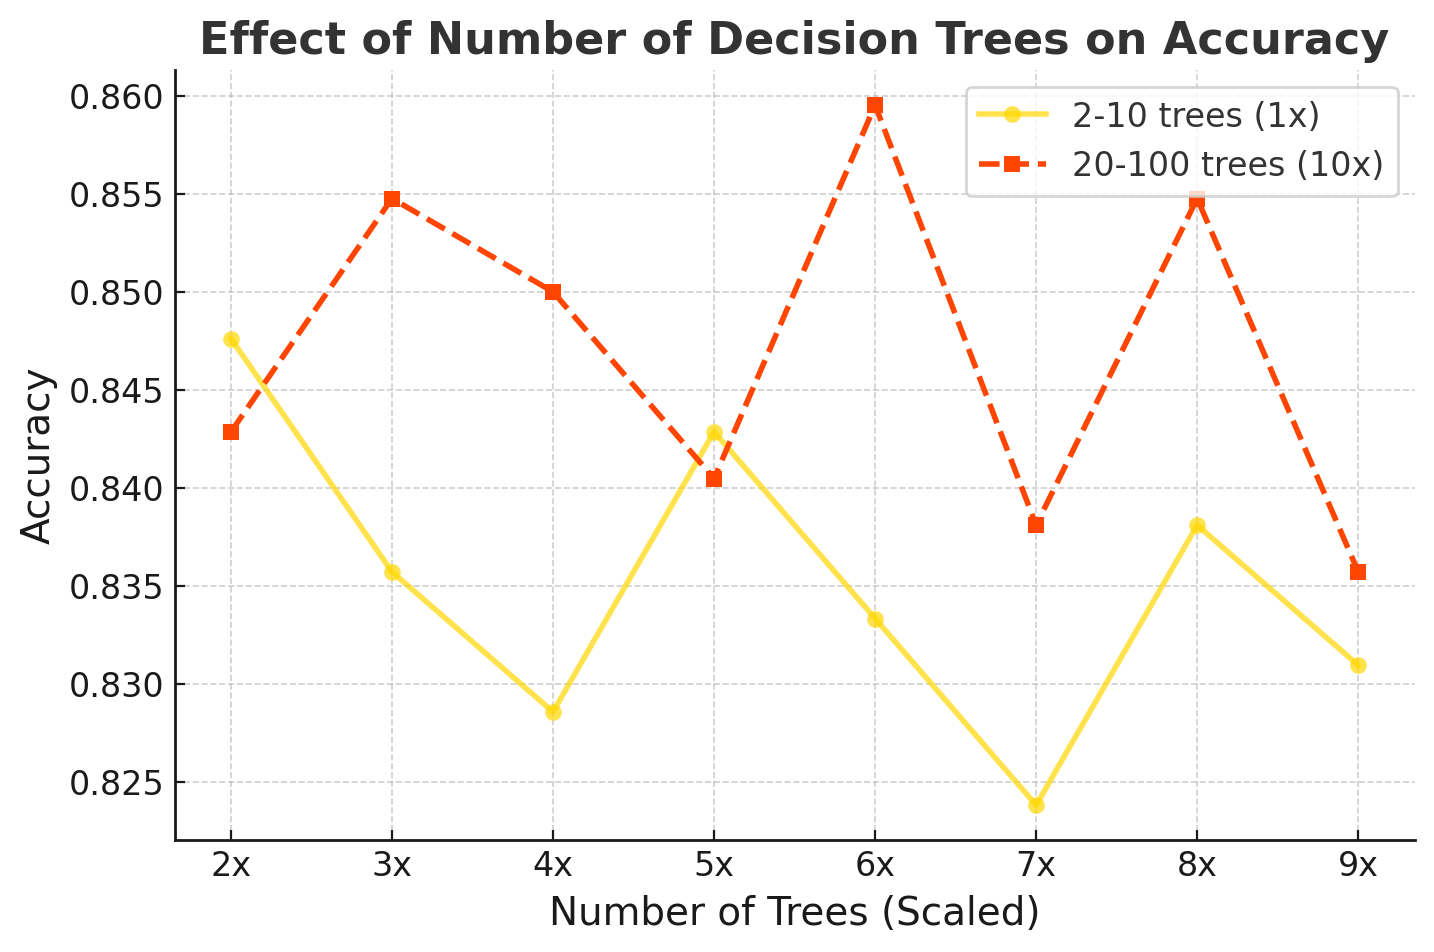
\includegraphics[width=0.8\textwidth]{src/picture3.png}
        \caption{隨機森林測試結果}
    \end{figure}
    我建構2$\sim$10,20$\sim$100棵決策樹,每棵決策樹的最大深度為10,最小子葉數為5進行測試。
    黃色實線代表2$\sim$10棵決策樹的準確率;橘色虛線則是20$\sim$100棵決策樹的準確率,以上的測試均使用20筆不同的測試資料取其平均。
    PS.由於隨機森林的取樣存在隨機性,因此我原本對於每組測試資料要建構10次隨機森林取平均,但這樣下來總共需要建構118800棵決策樹,
    我的筆電無法負荷這麼大的運算量(測試時執行了一個多小時才完成五分之一),因此我只建構了一次

    可以發現,即使是最差的狀況也有八成以上的準確率,能有效解決過擬合的問題。

    \newpage
    \section*{References}
    \begin{enumerate}
        \item https://medium.com/@SCU.Datascientist/python學習筆記-決策樹-decision-tree-b9acf11f0f84
        \item https://ithelp.ithome.com.tw/articles/10271143?sc=hot
        \item https://zh.wikipedia.org/zh-tw/決策樹學習
        \item https://blog.csdn.net/qq\_38502736/article/details/107210625
        \item https://github.com/mcxiaoxiao/c-Decision-tree
        \item https://zh.wikipedia.org/zh-tw/隨機森林
        \item https://ithelp.ithome.com.tw/m/articles/10272586
        \item ChatGpt(協助建立折線圖、表格、letex排版)
    \end{enumerate}


    \newpage
    \section*{Appendix}

    \subsection*{Tables of Decision Trees}

    %table 1
    \begin{table}[H]
        \centering
        \caption{使用決策樹,訓練資料與測試資料完全相同}\label{tab1}
        \vspace{1em}
        \begin{tabular}{ccc|ccc}
            \toprule
                最小子葉 &  最大深度 & 準確率 &  最小子葉 &  最大深度 & 準確率\\
            \midrule
            \hline
                3  &  5  &  73.79 \text{\%}  &  7  &  5  &  74.26 \text{\%}  \\
                3  & 10  &  86.12 \text{\%}  &  7  & 10  &  80.19 \text{\%}  \\
                3  & 15  &  89.39 \text{\%}  &  7  & 15  &  80.19 \text{\%}  \\
                3  & 20  &  89.39 \text{\%}  &  7  & 20  &  80.19 \text{\%}  \\
                4  &  5  &  74.10 \text{\%}  &  8  &  5  &  73.95 \text{\%}  \\
                4  & 10  &  85.02 \text{\%}  &  8  & 10  &  78.94 \text{\%}  \\
                4  & 15  &  86.12 \text{\%}  &  8  & 15  &  78.94 \text{\%}  \\
                4  & 20  &  86.12 \text{\%}  &  8  & 20  &  78.94 \text{\%}  \\
                5  &  5  &  74.10 \text{\%}  &  9  &  5  &  73.79 \text{\%}  \\
                5  & 10  &  83.62 \text{\%}  &  9  & 10  &  78.16 \text{\%}  \\
                5  & 15  &  83.93 \text{\%}  &  9  & 15  &  78.16 \text{\%}  \\
                5  & 20  &  83.93 \text{\%}  &  9  & 20  &  78.16 \text{\%}  \\
                6  &  5  &  73.95 \text{\%}  & 10  &  5  &  73.01 \text{\%}  \\
                6  & 10  &  81.90 \text{\%}  & 10  & 10  &  77.38 \text{\%}  \\
                6  & 15  &  81.90 \text{\%}  & 10  & 15  &  77.38 \text{\%}  \\
                6  & 20  &  81.90 \text{\%}  & 10  & 20  &  77.38 \text{\%}  \\
            \bottomrule
            \end{tabular}
    \end{table}

    %table 2
    \begin{table}[H]
        \centering
        \caption{使用決策樹,訓練資料與測試資料完全不同}\label{tab2}
        \vspace{1em}
        \begin{tabular}{ccc|ccc}
            \toprule
             最小子葉 &  最大深度 & 準確率 &  最小子葉 &  最大深度 & 準確率\\
            \midrule
            \hline
                3  &  5  &  60.71 \text{\%}  &  7  &  5  &  57.62 \text{\%}  \\
                3  & 10  &  60.24 \text{\%}  &  7  & 10  &  56.19 \text{\%}  \\
                3  & 15  &  60.24 \text{\%}  &  7  & 15  &  56.43 \text{\%}  \\
                3  & 20  &  60.71 \text{\%}  &  7  & 20  &  56.43 \text{\%}  \\
                4  &  5  &  58.33 \text{\%}  &  8  &  5  &  55.48 \text{\%}  \\
                4  & 10  &  58.57 \text{\%}  &  8  & 10  &  54.05 \text{\%}  \\
                4  & 15  &  57.38 \text{\%}  &  8  & 15  &  54.05 \text{\%}  \\
                4  & 20  &  57.38 \text{\%}  &  8  & 20  &  54.05 \text{\%}  \\
                5  &  5  &  58.57 \text{\%}  &  9  &  5  &  55.48 \text{\%}  \\
                5  & 10  &  59.05 \text{\%}  &  9  & 10  &  52.86 \text{\%}  \\
                5  & 15  &  58.57 \text{\%}  &  9  & 15  &  52.86 \text{\%}  \\
                5  & 20  &  58.57 \text{\%}  &  9  & 20  &  52.86 \text{\%}  \\
                6  &  5  &  57.14 \text{\%}  & 10  &  5  &  56.43 \text{\%}  \\
                6  & 10  &  56.19 \text{\%}  & 10  & 10  &  55.95 \text{\%}  \\
                6  & 15  &  56.90 \text{\%}  & 10  & 15  &  55.95 \text{\%}  \\
                6  & 20  &  56.90 \text{\%}  & 10  & 20  &  55.95 \text{\%}  \\
            \bottomrule
            \end{tabular}
    \end{table}

    \subsection*{Tables of Random Forests}

    %table 3
    \begin{table}[H]
        \centering
        \caption{使用隨機森林,訓練資料與測試資料完全不同}\label{tab3}
        \vspace{1em}
        \begin{tabular}{c c | c c}
            \toprule
            決策樹數量 & 準確率 & 決策樹數量 & 準確率 \\
            \midrule
            \hline
            2  & 0.847619  & 10  & 0.852381  \\
            3  & 0.835714  & 20  & 0.842857  \\
            4  & 0.828571  & 30  & 0.854762  \\
            5  & 0.842857  & 40  & 0.850000  \\
            6  & 0.833333  & 50  & 0.840476  \\
            7  & 0.823810  & 60  & 0.859524  \\
            8  & 0.838095  & 70  & 0.838095  \\
            9  & 0.830952  & 80  & 0.854762  \\
            90 & 0.835714  & 100 & 0.838095  \\
            \hline
        \end{tabular}
    \end{table}

              
%the end of the document
%do not change lists below
\end{document}
